%! alt Square with B at the origin, C = (12, 0) on the x-axis and A = (0, 12) on the y-axis, and the fourth vertex D. Point P = (10/3, 5) lies below the diagonal AC. Triangles PAB and PBC are shaded with areas 20 and 30, and triangle PAC is highlighted with area 22.
%! after_paragraph 1
%! scale 1/3
% The shared preamble of every Cevian figure. pipeline/figures turns these colours into theme-aware paint,
% and refuses any other colour, so draw only with them:
%   figink (lines and labels), figaux (construction lines), figaccent (the object the argument turns on),
%   figtint and figaccenttint (light fills).
\documentclass[border=1.5pt]{standalone}
\usepackage{tkz-euclide}
\definecolor{figink}{RGB}{0,0,0}
\definecolor{figaux}{RGB}{85,85,85}
\definecolor{figaccent}{RGB}{192,57,43}
\definecolor{figtint}{RGB}{221,221,221}
\definecolor{figaccenttint}{RGB}{245,213,208}
% tkz-euclide's defaults draw circles, compasses and marks in 50% grey and fill points with a tint.
\makeatletter
\def\tkz@otherlinecolor{figink}
\def\tkz@euc@circlecolor{figink}
\def\tkz@euc@compasscolor{figink}
\def\tkz@euc@mkcolor{figink}
\def\tkz@mk@fill{figink}
\def\tkz@euc@pointfillcolor{figink}
\makeatother
\tkzSetUpLine[color=figink,line width=.7pt]
\tkzSetUpArc[color=figink,line width=.7pt]
\tkzSetUpCompass[color=figink,line width=.5pt]
\tkzSetUpPoint[color=figink,fill=figink,size=3.1pt]
\tikzset{
  every picture/.style={line cap=round,line join=round,color=figink},
  circle style/.append style={color=figink,line width=.7pt},
  aux/.style={color=figaux,line width=.45pt,dash pattern=on 2.6pt off 2pt},
  key/.style={color=figaccent,line width=1pt},
  mk/.style={color=figink,line width=.5pt},
  lbl/.style={color=figink,inner sep=2.2pt},
  len/.style={color=figink,inner sep=1.5pt,font=\small},
}

\begin{document}
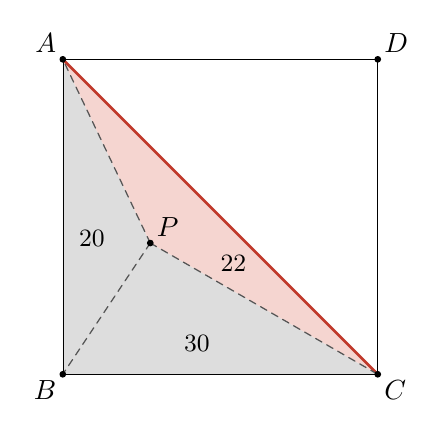
\begin{tikzpicture}
\tkzDefPoint(0.0,0.0){B} %! B = (0, 0)
\tkzDefPoint(4.0000000,0.0){C} %! C = (12, 0)
\tkzDefPoint(4.0000000,4.0000000){D} %! D = (12, 12)
\tkzDefPoint(0.0,4.0000000){A} %! A = (0, 12)
\tkzDefPoint(1.1111111,1.6666667){P} %! P = (10/3, 5)
\tkzDefPoint(0.37037037,1.8888889){K} %! K = ((10/3 + 0 + 0) / 3, (5 + 12 + 0) / 3)
\tkzDefPoint(1.7037037,0.55555556){L} %! L = ((10/3 + 0 + 12) / 3, (5 + 0 + 0) / 3)
\tkzDefPoint(2.1666667,1.5666667){N} %! N = (13/2, 47/10)
%! fact area(P, A, B) == 20
%! fact area(P, B, C) == 30
%! fact area(P, A, C) == 22
\tkzFillPolygon[color=figtint](P,A,B)
\tkzFillPolygon[color=figtint](P,B,C)
\tkzFillPolygon[color=figaccenttint](P,A,C)
\tkzDrawPolygon(A,B,C,D)
\tkzDrawSegment[key](A,C)
\tkzDrawSegments[aux](P,A P,B P,C)
\tkzDrawPoints(A,B,C,D,P)
\tkzLabelPoint[above left,lbl](A){$A$}
\tkzLabelPoint[below left,lbl](B){$B$}
\tkzLabelPoint[below right,lbl](C){$C$}
\tkzLabelPoint[above right,lbl](D){$D$}
\tkzLabelPoint[above right,lbl](P){$P$}
\tkzLabelPoint[len](K){$20$}
\tkzLabelPoint[len](L){$30$}
\tkzLabelPoint[len](N){$22$}
\end{tikzpicture}
\end{document}
